\section{Single Thread CPU Experiments}

We evaluate our code generation framework on a small set of kernels of high relevance to the machine learning community. 
All benchmarks measure single threaded CPU performance and compare to the peak performance of the machine.

\subsection{Preamble: Driving Experiments}
\MLIR provides a set of bindings for Python that support IR creation and manipulation at a generic level.\footnote{\url{https://mlir.llvm.org/docs/Bindings/Python}}
The infrastructure described in this paper aims to facilitate multi-level metaprogramming and drove the design of these bindings.

We additionally provide a custom domain-specific language (DSL) embedded into Python, referred to as OpDSL. 
The purpose of OpDSL is to shift the API paradigm from constructing a compiler IR to expressing computation in a concise, human-readable and mathematically compelling form, that has shown successful with Tensor Comprehensions~\cite{vasilache2019next}.
Figure~\ref{fig:opdslexample} illustrates a type-polymorphic matrix multiplication in OpDSL.
\begin{figure}[h!tb]
\centering
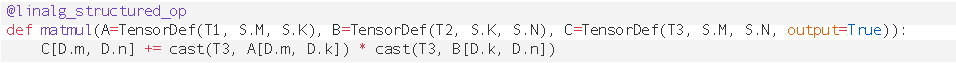
\includegraphics[width=\textwidth]{figures/opdsl_example_large}
\caption{Example: type-polymorphic matrix multiplication in OpDSL}
\label{fig:opdslexample}

\medskip
\centering
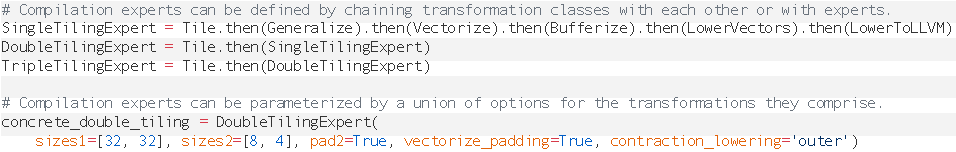
\includegraphics[width=\textwidth]{figures/tiling_experts_large}
\caption{Example: defining tiling transformations in Python}
\label{fig:tilingexample}
\end{figure}

The flow leverages and extends the minimal \MLIR execution engine for JIT-compilation and execution.
Structured data objects processed by the flow are exposed in Python as objects compatible with the Python buffer protocol.
They can therefore be converted to and from NumPy arrays, which are further convertible to framework-specific data types.
More details are given in Appendix~\ref{sec:appendix-python}.

In addition, we provide a test and benchmarking harness in Python to automate the measurement of compilation- and run-time as well as performance numbers such as $\mathrm{GFLOP}/s$ for computation and $\mathrm{GB}/s$ for memory traffic. 
The harness also wraps around the compilation and execution with multiple transformation strategies as described below.

\subsection{Preamble: Driving Transformations}
The transformations described in the previous sections are provided as configurable and callable ``transformation objects'' in Python.
These objects can be applied to \MLIR modules and perform the specified transformations on them.
Under the hood, the transformation results in a custom pass pipeline, consisting of the specified transformation pass with options set up as well as a handful of properly configured enabling/cleanup passes.
The pass pipeline is then run on the module.

The transformations currently available in Python are listed in Table~\ref{tbl:list-of-transformations}.
Certain transformations are applied in combination with tiling.
As discussed previously, the general notion of multi-dimensional subset --- applied to tensors, vectors, memrefs --- is load-bearing in our approach.
Transformations initially introduced on classical loops are generalized to multi-dimensional structured operations with the explicit goal of preserving structure.
Transformations may not be applicable until some loops are materialized by tiling as a means of explicitly and selectively discarding some parts of the structure.
In turn this improves the composition of transformations written as patterns: the matching conditions do not trigger until prerequisites are met.
For example, interchange applies to \emph{the loops produced by tiling} around the target structured operation.
Similarly, peeling only occurs on partial tiles.
Peeling and padding (Section~\ref{subsec:padding-values-and-packing}) are used as a means to ensure the main operations become fixed-shape and more easily amenable to vectorization (Section~\ref{subsec:vectorization}).

\begin{table}[h!tb]
    \centering
    \footnotesize
    \begin{tabularx}{\textwidth}{l|X}
    \toprule
    \textbf{Transformation} & \textbf{Options} \\\midrule
    \textsc{Tile} & \texttt{sizes} --- array of tile sizes \\
    ~ & \texttt{interchange} --- order of loops after tiling \\
    ~ & \texttt{pad} --- whether to pad partial tiles\\
    ~ & \texttt{pack\_paddings} --- non-removable padding for arrays\\
    ~ & \texttt{hoist\_paddings} --- number of loops from which to hoist padding for arrays\\
    ~ & \texttt{peel} --- loops from which to peel off partial tiles\\
    ~ & \texttt{scalarize\_dyn\_dims} --- whether to emit scalar code for non-vectorizable (dynamic) dimensions\\
    \hline
    \textsc{Vectorize} & \texttt{vectorize\_padding} --- whether to vectorize pad operations\\
    \hline
    \textsc{PipelineOneParentLoop} & \texttt{parent\_loop\_num} --- which parent loop to pipeline\\
    ~ & \texttt{II} --- Iteration Interval \\
    ~ & \texttt{read\_latency} --- Latency of a read operation \\
    \hline
    \textsc{UnrollOneParentLoop} & \texttt{parent\_loop\_num} --- which parent loop to unroll\\
    ~ & \texttt{unroll\_amount} --- by how many iterations to unroll the loop \\
    \hline
    \textsc{UnrollOneVectorOp} & \texttt{source\_shape} --- source shape of the vector op to unroll\\
    ~ & \texttt{source\_shape} --- target shape to unroll the vector op to \\
    \hline
    \textsc{Bufferize} & \emph{none}\\
    \hline
    \textsc{Sparsify} & \emph{none}\\
    \hline
    \textsc{LowerVectors} & \texttt{contraction\_lowering} --- how to lower vector contractions (outer/inner product, LLVM matrix intrinsics)\\
    ~ & \texttt{multi\_reduction\_lowering} --- how to lower multidimensional reductions (inner or outer parallel)\\
    ~ & \texttt{transpose\_lowering} --- how to lower transpositions (elementwise, flat, vector shuffle, target-specific)\\
    \hline
    \textsc{LowerToLLVM} & \emph{none}\\
    \bottomrule
    \end{tabularx}
    \smallskip
    \caption{\label{tbl:list-of-transformations}Transformations (and their options) that are currently available in Python. Some loop transformations apply only to loops produced by tiling and must be combined with tiling (e.g., peeling or interchange).}

  \medskip
  \footnotesize
  \centering
  \begin{tabularx}{\textwidth}{X|ccccccc}
    \toprule
     \textbf{Benchmark}             & L1 @ 12.8KB & L2 @ 20\% & L2 @ 40\% & L2 @ 90\% & L3 @ 40\% & L3 @ 80\% & DRAM \\
    \midrule
        copy (1 read + 1 write / B) &     289.5   &    89.3   &    83.9     &    54.8   &   25.7    &   17.2    &  12.2 \\
    \hline
   \begin{tabular}{@{}l@{}}extrapolated \\ (2 reads + 1 write / B)\end{tabular} &    434.25  &    134    &   125.8   &    82.2   &   38.5    &   25.8    &  18.3 \\
    \bottomrule
  \end{tabularx}
  \smallskip
  \caption{Measured and extrapolated single core copy performance in $\mathrm{GB}/s$.}
  \label{tbl:measured-bandwidths}
\end{table}

The transformations listed in Table~\ref{tbl:list-of-transformations} latch on a structured unit of the IR, with additional information and constraints.
E.g.\ for the \lstinline|UnrollOneVectorOp| case, the structured unit is \lstinline|vector.contract|, with additional constraints on its current shape, and providing the target shape after transformation.
Note that this direct control of multi-dimensional structured operations is not available in IRs that treat loops as the unit handle for transformations~\cite{ragan2013halide, chen2018tvm, vasilache2019next}.

To complete the environment to control and run transformation and code generation experiments, we provide a computation chaining API to define transformation sequences, see Figure~\ref{fig:tilingexample}.
% Together with Python metaprogramming, harnesses and interoperability capabilities, this provides a flexible, all-batteries-included environment to devise, control and run experiments.

\subsection{Experimental Setup}

Experiments are run on an Intel Xeon Gold 6154 CPU @ $3.00\mathrm{GHz}$.
This is a processor with dual-issue AVX512 fma instructions and 32KB of L1D, 32KB of L1I, 1MB L2 cache per core and a unified 25MB L3 shared by 18 cores.
Single-threaded single precision computations peak at $192\mathrm{GFLOP}/s$ 
(2 \lstinline|fma| operations per cycle, 2 operations (\lstinline|mul| + \lstinline|add|) each on 16 \lstinline|f32|).
The theoretical L1 bandwidth of a single core is $384\mathrm{GB}/s$ (assuming 1 load and 1 store instruction per cycle, each one of 64B).

Measurements are nearly bare-metal, in privileged mode, following scientific computing~\cite{benchmark2015} and LLVM benchmarking recommendations~\cite{LLVM_benchmarking}.
In particular, we disable turbo boost, address space randomization and the SMT pair of the core we run on.
We also run in a specific shielded \lstinline|cpuset| consisting of a single core and migrate all 
processes away from the core we execute on.

We further measure a peak memory bandwidths given in Figure~\ref{tbl:measured-bandwidths} with a simple contiguous copy benchmark.
We report the highest measured L1 throughput in $\mathrm{GB}/s$ which we find by fine-tuning, this maximum occurs for $12.8\mathrm{KB}$ read buffer size (i.e.\ $25.6\mathrm{KB}$ total buffer sizes, or approximately 80\% of L1 capacity).
Allocations occur at 64B boundary to guarantee the absence of cache line splitting given the sizes and transformations considered 
for this peak bandwidth analysis.
% Other than 64B-aligned allocations, we do not control allocation to e.g. guarantee good associativity behavior.
Since the hardware can issue 2 loads and 1 store per cycle, we also extrapolate the ideal scaling of the 
measured bandwidth to the actual load/store mix of a given scenario (i.e.\ by mechanically scaling the peak bandwidth by up to 50\% over the one measured with the copy benchmark).
Depending on the benchmark, the roofline~\cite{roofline} is either the measured copy bandwidth (e.g.\ for transpose or reduction) or the extrapolated bandwidth (e.g.\ for depthwise convolution that perform multiple reads for 1 write).
                            
In the following, all experiments consist of single threaded execution times measured on our benchmark system. 
We perform 100 measurements and plot the median. Black error bars show the 25\% and 75\% quantiles to quantify the measurement variance.
We report steady-state performance after dropping warm-up iterations due to compulsory cache misses and other overheads.\footnote{Note that with AVX-512, due to throttling issues, significant warmup may be required.}
Such overheads are relevant in larger-scale experiments in which fusion would be required to keep the L1 hot.
We compare the benchmark results to reference implementations to guarantee correctness.

\subsection{Benchmarks}

We evaluate the effectiveness of the strategies developed within our infrastructure on a range of kernels that dominate the execution time of machine learning workloads. All kernels execute a single tensor algebraic operation. Our results highlight the raw operator performance, independently of fusion and layout optimization opportunities across multiple operations.

We distinguish between memory-bound and compute-bound kernels. The memory-bound kernels move and reorder data to match the access patterns of the more compute intense operations. We benchmark the following memory-bound kernels:
\begin{itemize}
    \item Copy performance is an essential performance metric. The \emph{Copy2D} benchmark operates on $2$-D tensors that store contiguous data. This setup allows us more flexibility in targeting tiling, vectorization and unrolling than a flat $1$-D buffer but is otherwise equivalent.
    \item Transposition is a ubiquitous operation that comes in different shapes and sizes. The \emph{Transpose2D} benchmark implements a $2$-D transpose. It is the common denominator of higher dimensional transpose operations since a $n>2$-D transpose can be rewritten as iterated $2$-D transposes at various locations within the tensor. For instance a $4$-D $i,j,k,l\xrightarrow{} k,j,l,i$ transposition can be rewritten as $j\times k$ transposes of $(i,\ldots,l\xrightarrow{}\ldots,l,i)$. 
    This is always possible while keeping the fastest varying dimensions contiguous for both input and output tensors. 
    \item Reductions are data aggregation operations and an important algorithmic motif. Here we focus on the bandwidth-bound reductions associated with matrix-vector products or similar operations occurring in data analytics and neural networks. 
    The \emph{ColRed2D} and \emph{RowRed2D} benchmarks reduce the rows or columns of a $2$-D tensor to a $1$-D tensor, respectively. 
\end{itemize}

Compute-bound kernels have significant reuse and exhibit much higher computational than memory bandwidth needs. 
Their execution time is thus limited by the compute throughput rather than the memory bandwidth.
We benchmark the following compute-bound kernels:
\begin{itemize}
\item Matrix multiplication is ubiquitous in numerical computing. 
  The \emph{Matmul} benchmark implements plain matrix multiplication.
\item Convolutions ($1$-D and $2-D$ with strided and dilated variants) dominate
  the execution time of many machine learning models. In this paper we focus on 
  the so-called \emph{NHWC} format but other formats are trivial to generate with
  our OpDSL approach.
\end{itemize}
Lastly, we discuss the performance of depthwise convolutions for sizes relevant to the popular MobileNet~\cite{MobileNetV2} model.
\emph{DepthwiseConv2D} is a \emph{NHWC} format kernel whose compute to communication ratio presents challenging and interesting problems. 

For each benchmark, we manually derive up to 5 expert compiler strategies using the transformations of Table~\ref{tbl:list-of-transformations}. 
In each case, we run a few manual experiments to devise good register tile sizes such that the performance of L1-resident kernels is high.
We then fix the tile sizes and select the best performing strategy among the 5 in each case.
This is akin to a fixed expert-driven heuristic.

Systematic autotuning and search space exploration is an area of active investigation that is expected to bring significant improvements.
We discuss preliminary results with autotuning in Section~\ref{subsec:prelim-tuning-results}.

\subsection{Performance of Memory-Bandwidth-Bound Kernels}

A bandwidth-bound kernel may be limited by different levels of the memory hierarchy, depending on problem size and access pattern. 
We run the bandwidth-bound kernels on different problem sizes and analyze their performance for all three cache hierarchy levels. 
In the particular case of the \lstinline|copy| benchmark, we run a small search over different $2$-D vector sizes, load/store interleaving, and loop unrolling specific for every problem size.
The measured bandwidth then becomes our L1 bandwidth measuring stick.

\subsubsection{L1 Bandwidths}
\autoref{fig:l1-bandwidth} shows the achieved memory bandwidth for all bandwidth-bound kernels on problem sizes fitting L1 cache. 
We observe the highest bandwidths for the \emph{Copy2D} kernel that performs exactly $1$ \lstinline|vector.load| and $1$ \lstinline|vector.load| per 64B of data. 
This kernel does not perform any computation nor rearranges data. 
Despite executing in a tight loop with data resident in L1 cache, the benchmarks show that offsetting latency requires a sufficiently large problem size. 
We start seeing L1 bandwidth performance in the 200 GB/s zone only at around 4KB of read data (8KB total, i.e.\ 25\% L1 capacity).
A 200GB/s L1 bandwidth is sustained only in the 8KB--14KB range of read data (16KB--28KB total, i.e.\ 50-87\% L1 capacity).
We observe the maximal bandwidth of 289 GB/s at roughly 75\% L1 cache utilization. 
Larger problem sizes achieve lower bandwidths, presumably, due to conflict misses.
Lastly, variance starts increasing greatly around 80\% of L1 capacity.

\begin{figure}[h!tb]
\centering
\minipage[t]{\textwidth}
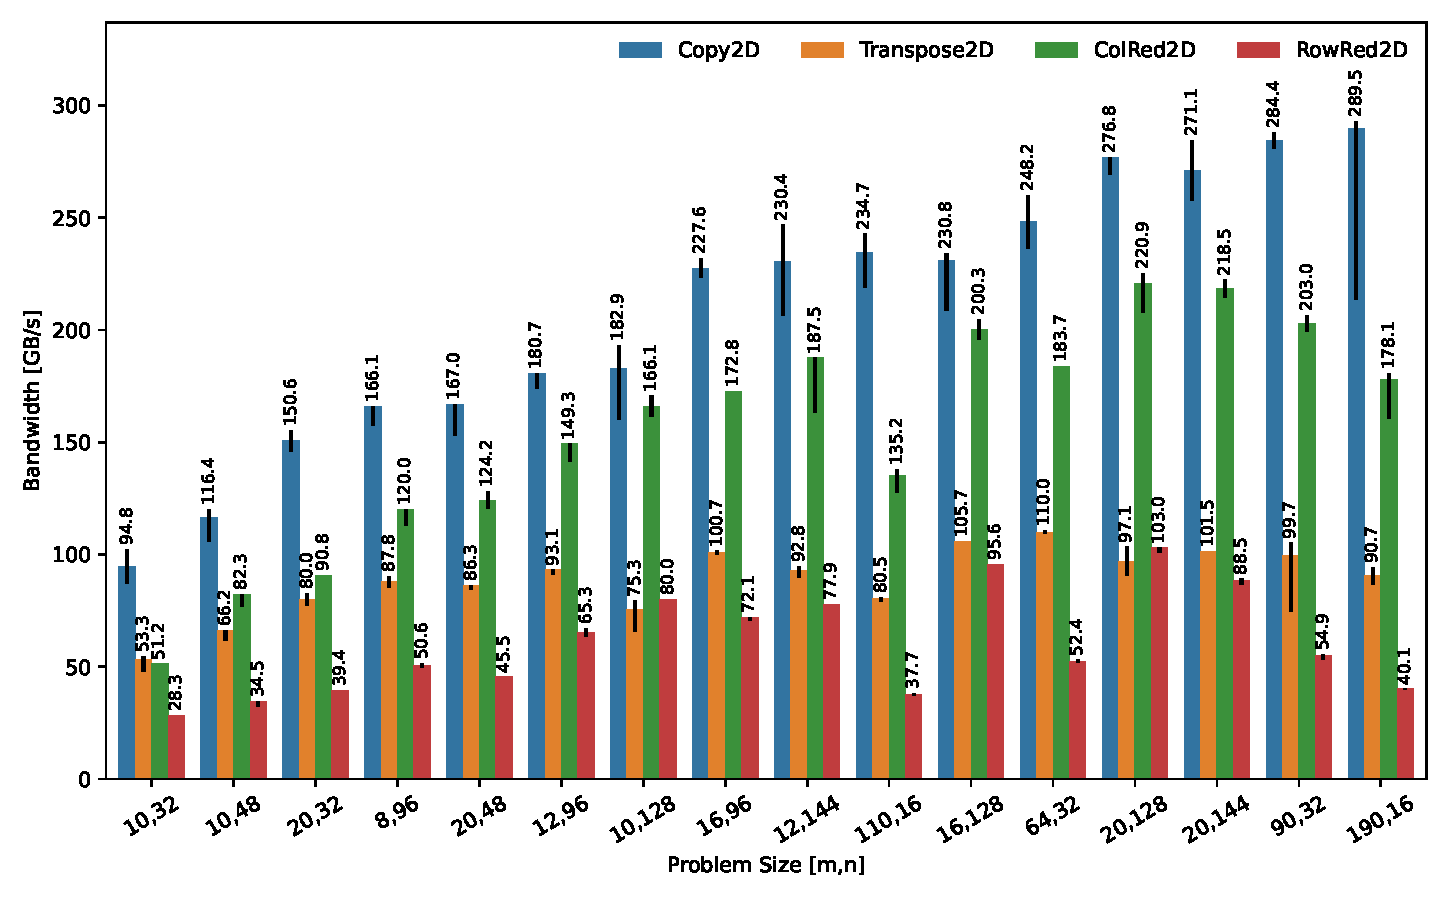
\includegraphics[width=0.98\textwidth]{plots/bandwidth/bandwidth-bound-l1.pdf}
\endminipage
\caption{\label{fig:l1-bandwidth}Memory bandwidth for bandwidth-bound kernels on problem sizes fitting L1 cache. Theoretical copy peak bandwidth is 384 GB/s (289 GB/s measured). Transpose performance is limited by \lstinline|xmm| loads and \lstinline|ymm| shuffles, more work is needed to get good \lstinline|zmm| assembly (see Section~\ref{subsubsec:transpose-discussion}).}
\end{figure}

\emph{Transpose2D} rearranges the data while moving.
This results in significantly more complex instruction sequences than a \emph{Copy2D}'s simple $1$ load $1$ store pattern.
We achieve bandwidths of 30-60\% of \emph{Copy2D} and up to 109 GB/s L1 bandwidth for the most favorable size.
We discuss the characteristics of this kernel more deeply in Section~\ref{subsubsec:transpose-discussion} as well as opportunities for improvement.

\emph{ColRed2D} and \emph{RowRed2D} read more data (a full $2$-D tensor) than they write (a $1$-D tensor).
This is beneficial on our test system that can perform $2$ reads and $1$ write per cycle (see Table~\ref{tbl:measured-bandwidths}).
At the same, time they perform computations.
In particular \emph{RowRed2D} performs an expensive horizontal reduction along the vectorization dimension. 
While \emph{ColRed2D} achieves high bandwidths of up to 212 GB/s, we observe only up to 99 GB/s for \emph{RowRed2D}.
The lower performance is particularly pronounced for problem sizes with a short reduction dimension. 
This is due to the mapping of horizontal reduction on Intel processors and the notorious cost of crossing \lstinline|ymm| and \lstinline|xmm| boundaries.
The resulting performance is not better than combining \emph{Transpose2D} and \emph{ColRed2D}.
Finer tuning and better AVX-512 patterns are expected to improve the situation in the future.

%
Overall, rearranging data or performing computation during data movement immediately reduces the achieved L1 cache bandwidth.

\subsubsection{L2 Bandwidths}
\autoref{fig:l2-bandwidth} shows the achieved memory bandwidths for problem sizes fitting L2 cache. 
\emph{ColRed2D} and \emph{RowRed2D} achieve the highest bandwidths due to their favorable read-to-write ratio. 
We observe bandwidths of up to 125 GB/s. 
\emph{RowRed2D} achieves similarly high bandwidth but also falls behind for problem sizes with small vector dimension, due to the slow reduction of the last vector in the row. 
%
The difference between \emph{Copy2D} and \emph{Transpose2D} is less pronounced since the cost for rearranging the data partly overlap with the slower data movement.

\begin{figure}[h!tb]
\centering
\minipage[t]{\textwidth}
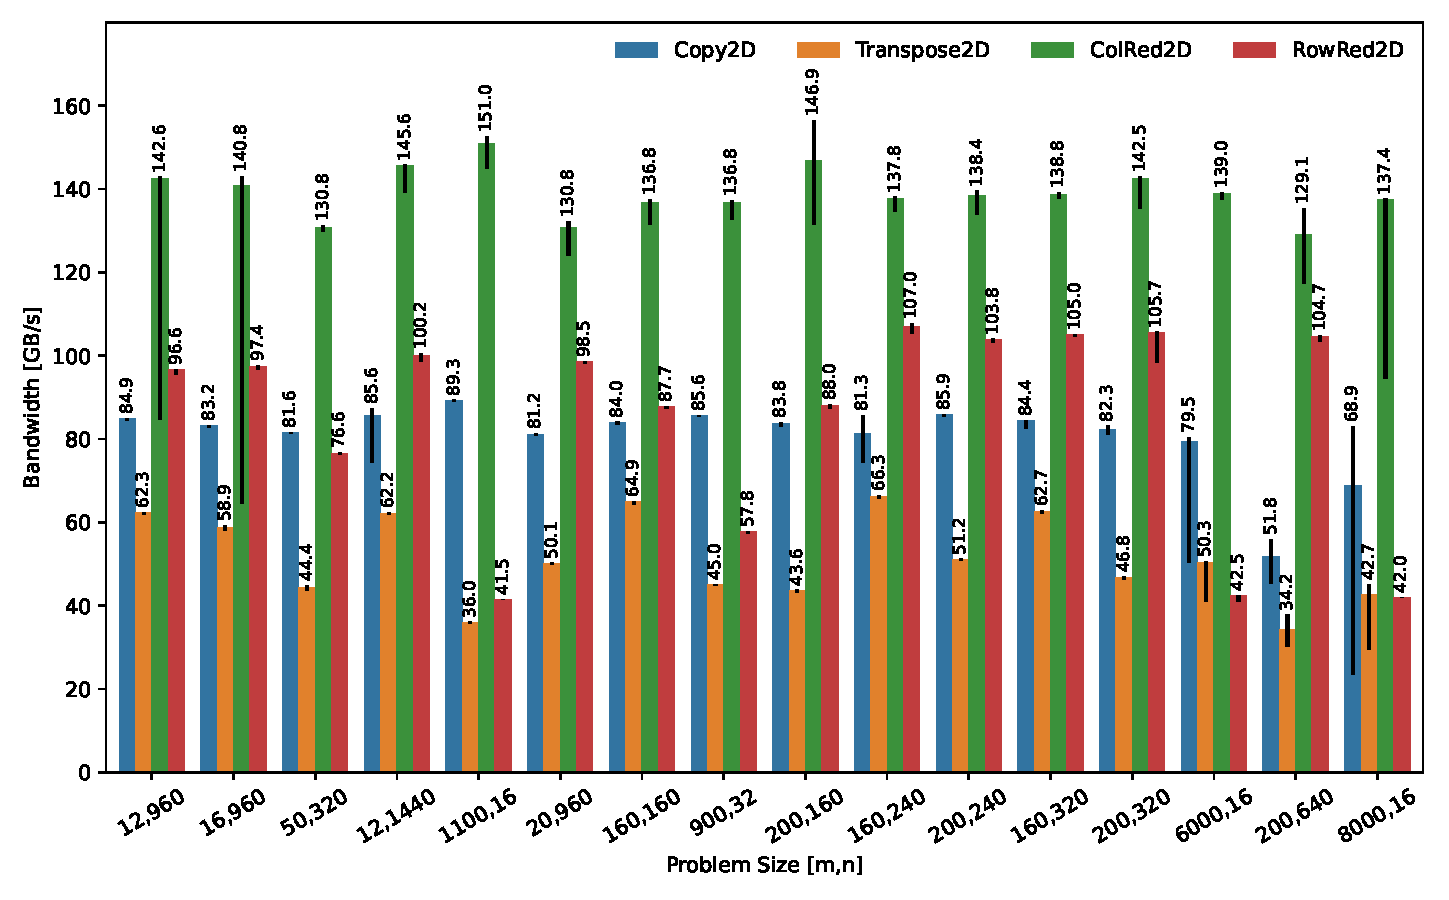
\includegraphics[width=0.98\textwidth]{plots/bandwidth/bandwidth-bound-l2.pdf}
\endminipage
\caption{\label{fig:l2-bandwidth}Memory bandwidth for bandwidth-bound kernels on problem sizes fitting the L2 cache. 
Measured peak copy bandwidth is $83.9 \mathrm{GB}/s$ ($1$ read and $1$ write per byte). 
Reductions can go past this because they perform an amortized $2$ reads and a fraction of a write per iteration. 
Despite the extra compute, dropping most writes is still a net win.}
\end{figure}

\subsubsection{L3 Bandwidths}
\autoref{fig:l3-bandwidth} shows the achieved memory bandwidths for problem sizes fitting L3 cache. 
All benchmarks except for \emph{Transpose2D} peak at an achieved memory bandwidth of 26 GB/s. 
We attribute this performance difference to the L3 cache latency of that cannot be hidden for the transpose access patterns.

\begin{figure}[h!tb]
\centering
\minipage[t]{\textwidth}
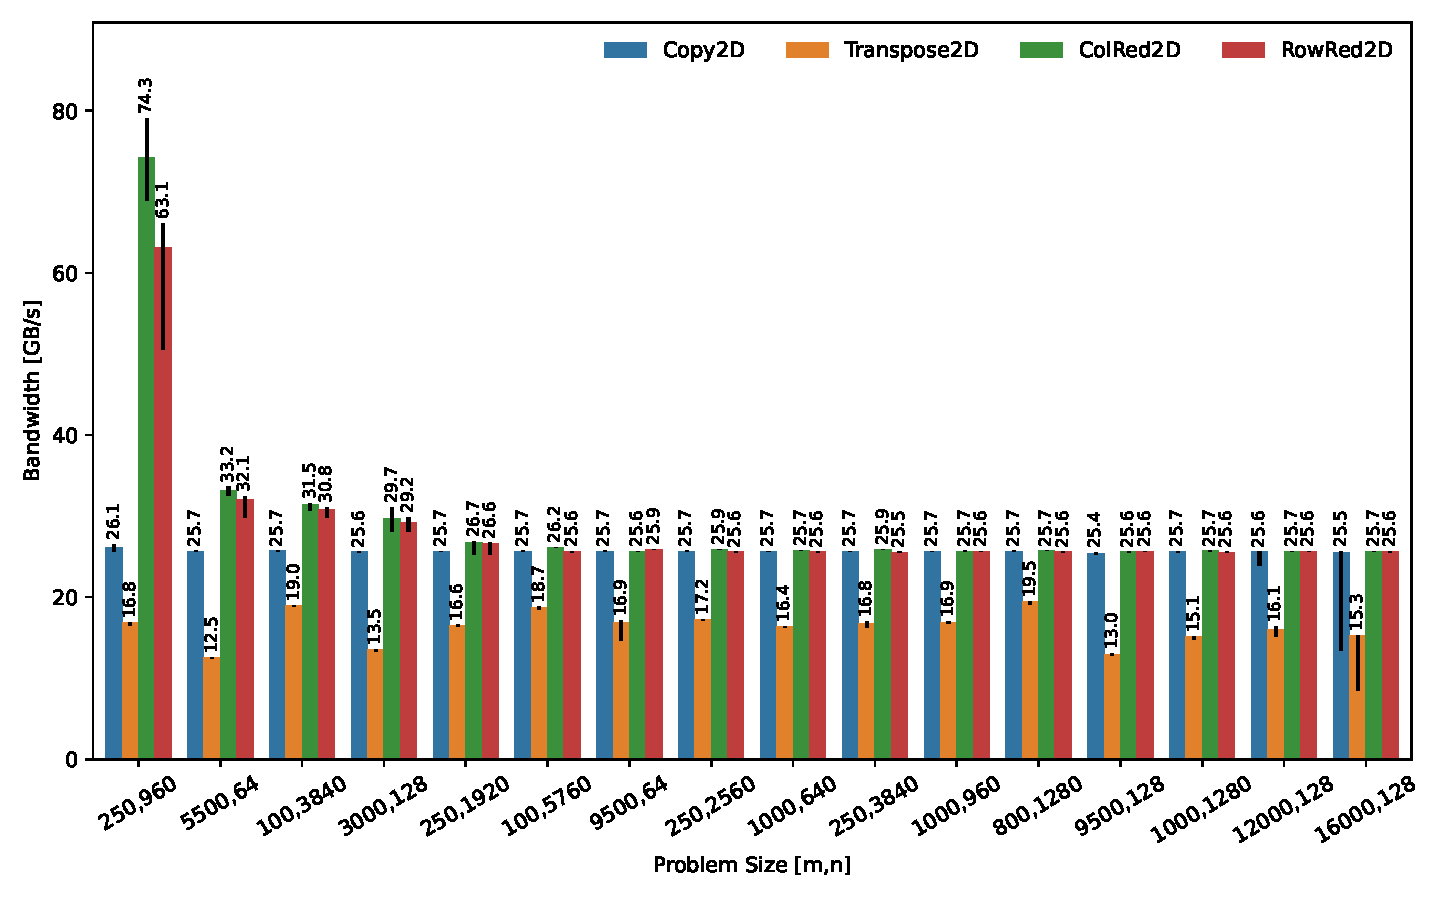
\includegraphics[width=0.98\textwidth]{plots/bandwidth/bandwidth-bound-l3.pdf}
\endminipage
\caption{\label{fig:l3-bandwidth}Memory bandwidth for bandwidth-bound kernels on problem sizes fitting L3 cache. 
Measured copy peak is 25.7 GB/s (L3 @40\%). 
Note that reductions of 250x960xf32 still fit in L2 because the write buffer is much smaller 
(i.e. \lstinline|250xf32| for row reduction and \lstinline|960xf32| for columns reduction.}
\end{figure}

\subsubsection{Transpose Discussion}
\label{subsubsec:transpose-discussion}
In this section, we dive deeper into the specific performance of the transpose
patterns we generate and discuss opportunities for improvements.

First, to get to the best transposed version, the Intel Reference Optimization Manual~\cite{IntelOptimizationManual} recommends using the \lstinline|vblendps| instruction (example 15.19).
The vector dialect provides a dedicated \lstinline|vector.transpose| operation as well as multiple lowering strategies when going to LLVM. 
Since we emit LLVMIR, we do not have direct control over register allocation and instruction selection.
To offset this lack of control, hardware-specific vector dialects (e.g. the \lstinline|x86vector| dialect) provide
access to intrinsics to match clang intrinsics such as \lstinline{_mm256_blend_ps}.
Unfortunately, some of these clang intrinsics (including \lstinline{_mm256_blend_ps}) are not backed by a real intrinsic 
implementation and do not provide direct access to the corresponding ISA.
Instead, they lower immediately to generic LLVM \lstinline|shufflevector| instructions!
LLVM then relies on peephole optimization and especially \emph{SelectionDAG}; but these contain ``very little
arch-specific shuffle combines''~\cite{VBlendPsLimitation}.
In such a case, we were not able to compile to the desired \emph{vblendps} operation. 
Instead, we had to originally settle to a pure shuffle-based implementation\footnote{Note that such a pure shuffle-based 
implementation is similar to the one used in the
Eigen~\cite{eigen} library (more specifically, the \lstinline|ptranspose(PacketBlock<Packet8f,8>& kernel)| routine).}.

To circumvent this issue, we also provide an \lstinline{InlineAsmOp} and specific asm-based intrinsics that encode
the intended instructions (e.g. an \lstinline{mm256BlendPsAsm} lowering helper that is \emph{guaranteed} to emit the \lstinline{vblendps} instruction where we intend it to)\footnote{
We provide such specialized avx2 lowerings under the \lstinline|transpose\_lowering=avx2| for \lstinline|vector| transpose
of size \lstinline|8x8|.}.
This provides a nice \lstinline|30-40\%| performance boost on small transpose sizes over the version
generated by LLVM for an 8x8 transpose implemented only with intrinsics that lower to \lstinline|shufflevector|.

The Intel Reference Optimization Manual~\cite{IntelOptimizationManual} further recommends using specific permutation instructions from memory to further reduce shuffle issue port pressure.
These are not yet available as first-class citizens in our lowering but LLVM's peephole optimization was able to recover the
pattern in the very specific case of a \lstinline|4x8| tiling of the transpose.
While this does not make use of \lstinline|avx512| instructions and is thus potentially 2x slower 
than we could hope for, the LLVM  \lstinline|4x8| version performs best, by far.
We summarize our findings in Table~\ref{tbl:comparison-transpose}.

\begin{table}[h!tb]
  \small
  \centering
  \begin{tabularx}{\textwidth}{X|cccc}
    \toprule
    \textbf{Size}     & \textbf{Tile8x8Shuffle}  & \textbf{Tile16x16Shuffle} & \textbf{Tile8x8AVX2} & \textbf{Tile4x8Shuffle}  \\
    \midrule
    \lstinline|16x16| &          24.1     &       22.5       &     41.8    &      55.3     \\
    \hline
    \lstinline|32x32| &          29       &       27         &     64      &      95       \\
    \bottomrule
  \end{tabularx}
  \smallskip
  \caption{Median (p50) measured performance of a \lstinline|vector.transpose| lowering strategies (GB/s).
   The "natural" \lstinline|16x16| native AVX512 lowering with \lstinline|shufflevector| performs significanly
   worse than a custom \lstinline|8x8| AVX2 lowering mixing \lstinline|vblendps| and \lstinline|shufflevector|.
   The less obvious \lstinline|4x8| tiling and \lstinline|shufflevector| performs significantly better despite
   using \lstinline|xmm| loads.}
  \label{tbl:comparison-transpose}
\end{table}

Based on this understanding, we conducted additional experiments using \lstinline|UnrollOneVectorOp| 
to try and keep a \lstinline|16x16| \lstinline|vector.transpose| shape while forcing \lstinline|xmm| and \lstinline|ymm| loads. 
This experiments resulted in a performance degradation, likely due to the \lstinline|shufflevector| that we do not yet canonicalize. 
More work will be needed to get to the bottom of  this. 

The performance has room for future improvements as we devise a better-suited AVX512 version and more finely tune tile sizes and codegen strategies.
We expect a better AVX512 solution will likely involve insight from prior work on Knight's Landing~\cite{IPDPS2013}.
For now, the measured efficiency is between 30\% and 55\% for a fully isolated $2$-D transpose operation.
This has to be put in additional context.
The copy kernels we studied in the previous section perform exactly $1$ 64B load and $1$ 64B store for each operation.
The transpose kernels are significantly more complex.
They involve 16B and 32B loads but still reach a comparatively high performance, given the small loads and additional shuffle instructions.

Lastly, an additional argument to consider is that transpositions are by themselves rarely isolated in a vacuum.
Instead, they often compose with other operations (e.g. matmul), in which case their cost is often amortized.

\subsection{Performance of Compute-Bound Kernels}

Let us now review the performance of matrix multiplication and convolutions.

\subsubsection{Matrix Multiplication}

Attaining a high matrix multiplication throughput is essential in numerical computations. 
We measure the performance for plain matrix multiplication and transposed variants:
\begin{equation*}
\begin{split}
C[m,n] = A[m,k]B[k,n] & \qquad(AB) \\
C[m,n] = A[k,m]B[k,n] & \qquad(A^TB) \\
C[m,n] = A[m,k]B[n,k] & \qquad(AB^T)
\end{split}
\end{equation*}

\begin{figure}[h!tb]
\centering
\minipage[t]{\textwidth}
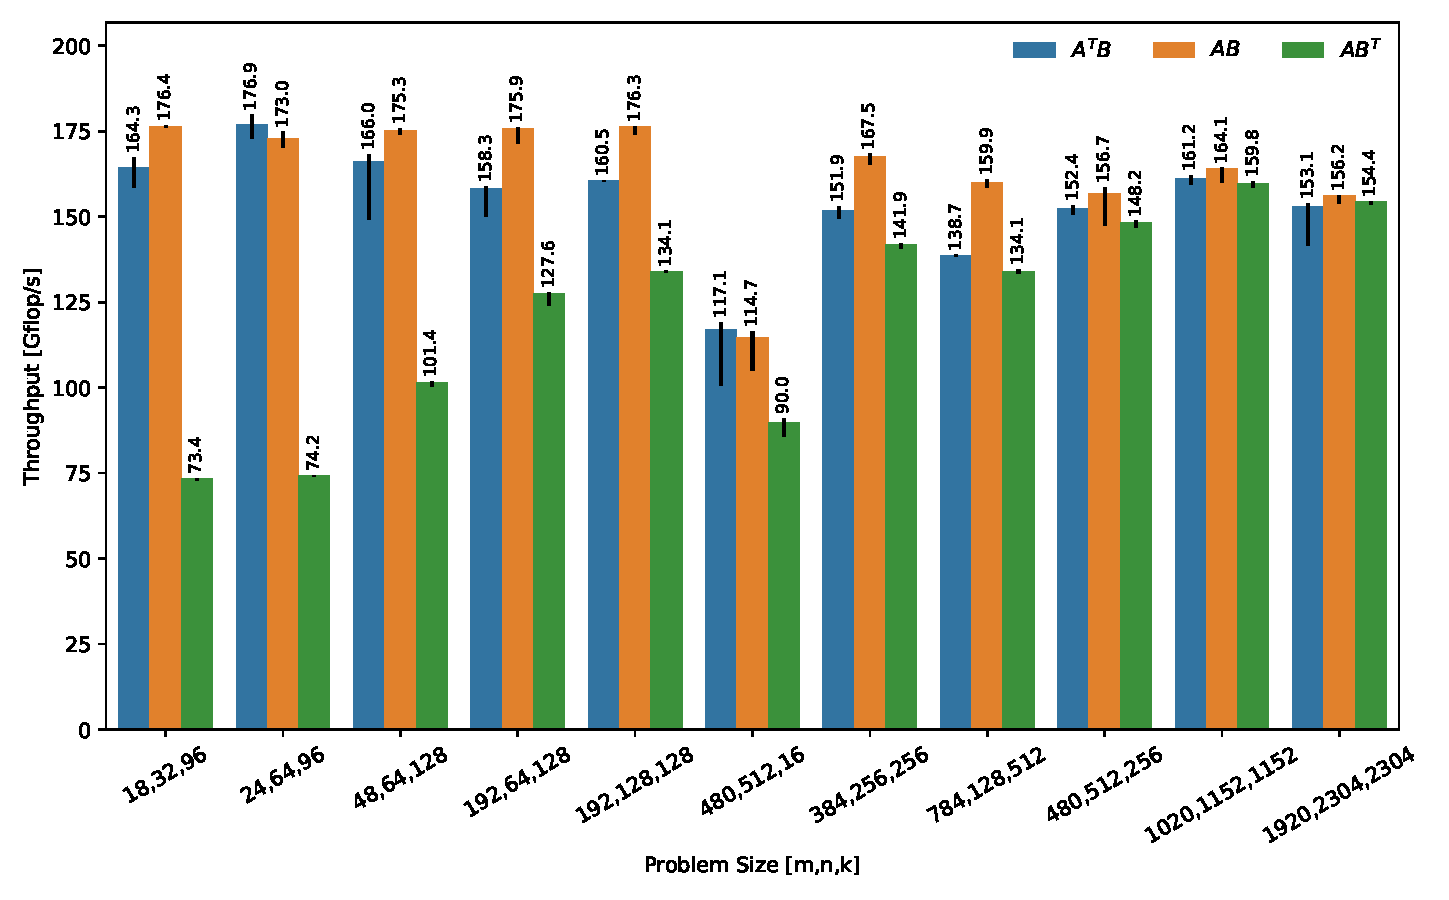
\includegraphics[width=0.98\textwidth]{plots/matmul/matmul.pdf}
\endminipage
\caption{\label{fig:matmul}Matrix multiplication compute throughput for different storage layouts and problem sizes (best of 5 fixed strategies). The theoretical peak is $192 \mathrm{GFLOP}/s$, fine peformance tuning is left for future work.}
\end{figure}

Figure~\ref{fig:matmul} illustrates the performance of matrix multiplication for various sizes. 
We reach a 92\% efficiency in the \lstinline|AB| kernel case, which demonstrates that our codegen approach emits close to peak arithmetic intensity kernels.
It is worth noting that in the low-latency regime cases, layout has a significant impact on performance.
In particular, the $AB^T$ has a significantly lower performance due to the layout of reduction dimension along the fastest varying memory dimension (i.e.\ $C[m,n] = A[m,k]B[n,k]$). 
This is a similar horizontal reduction issue as for \emph{RowReduction2D}.
At low-latency sizes, the cost of a transpose is prohibitive and performance suffers. 
As we reach larger sizes, the tranpose becomes beneficial and no more performance difference is observable. 

Larger sizes use a fixed tiling of \lstinline|288x128x512| but are not specifically tuned.
Additionally, we do not yet emit prefetch instructions or try to pipeline data movements with computation. 
These transformations along with deeper tuning is left for future work.
For a preview discussion of achievable performance combining autotuning with our infrastructure, see Section~\ref{subsec:prelim-tuning-results}.

\subsubsection{Convolution}

Convolution folds an input tensor with a multi-dimensional kernel following a \emph{sliding window} pattern.
%\ntv{note, I dropped the "image" terminology because in 1-D these are typically signals (e.g. sound)}.
We specify a convolution operator in terms of its input image and kernel dimensions following standard practice in the ML literature:
\begin{itemize}
 \item $H$: height of the image,
 \item $W$: width of the image,
 \item $N$: batch number of the image (input and output only),
 \item $C$: input channels of the image,
 \item $F$: output filters of the image (kernel only),
\end{itemize}
Additional parameters are the kernel widths $K_h$ and $K_w$, the strides $S_w$ and $S_h$, and the dilations $D_w$ and $D_h$. We measure the performance for $1$-D and $2$-D convolution in \lstinline|NHWC| format:
\begin{equation*}
\begin{array}{llll}
O[n,w,f] &=& I[n,w\times S_w+k_w\times D_w,c]\cdot K[k_w,c,f] & (1-D) \\
O[n,h,w,f] &=& I[n,h\times S_h+k_h\times D_h,w\times S_w+k_w\times D_w,c]\cdot K[k_h,k_w,c,f] & (2-D)
\end{array}
\end{equation*}
where the stride ($S_h$ and $S_w$) and the dilations ($D_h$ and $D_w$) parameters control the input image access pattern. 

\autoref{fig:conv-1d} shows the compute throughput for the $1$-D (left) and the $2$-D (right) convolution after tiling once. 
All problem sizes not shown in the plot are constant ($(N,C,F,K_w)=(1,32,64,3)$ for the $1$-D case and $(N,C,F,K_w)=(1,32,64,3,3)$ for the $2$-D case).
The reader familiar with the literature may remark that we are providing performance results for the more difficult \emph{batch size 1} configuration.
The particularity of the problem is that it contains one fewer dimension of parallelism.

We measure high performance for both the $1$-D and the $2$-D convolution when the stride is $1$, with a peak at around $96\%$ of theoretical hardware peak.
We observe a slowdown for non-unit strides.
The slowdown is more pronounced in the $1$-D case where the data size is quite small and the computation do not make up for the loss in access pattern efficiency.
The inefficiencies start to dissipate above input size $40$ and almost disappear in the $2$-D case.
Note that sizes $20$ and $55$ are not perfect multiples of the good vector sizes and require multi-dimensional loop peeling, resulting in lower performance (padding is not beneficial at such small sizes)\footnote{Specific size tuning to avoid peeling along some dimensions is expected to further improve the performance in such cases.}.

\begin{figure}[h!tb]
\centering
\minipage[t]{\textwidth}
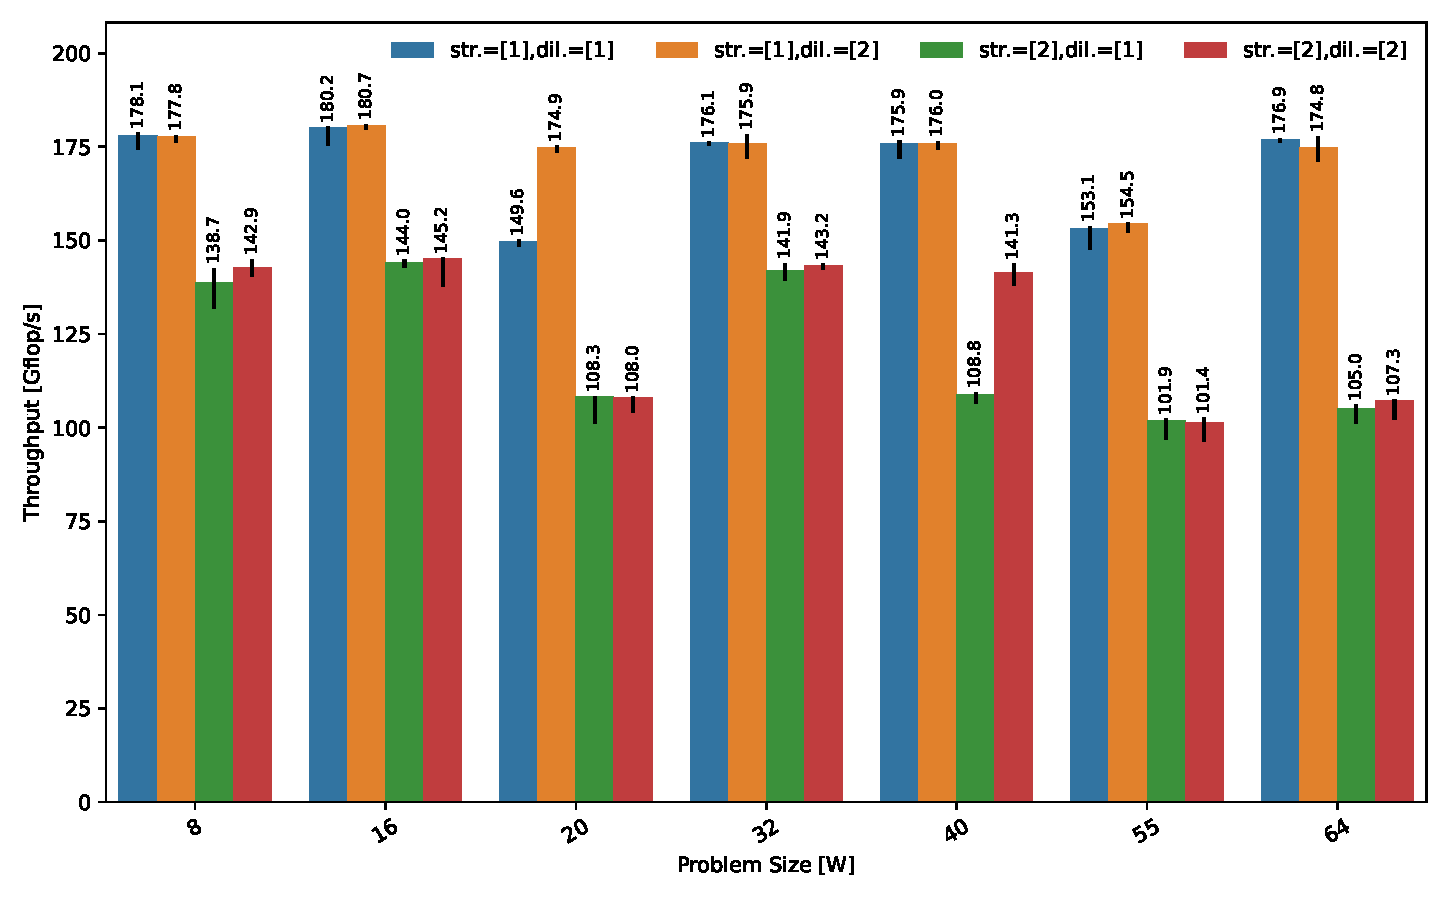
\includegraphics[width=0.98\textwidth]{plots/conv/conv_1d.pdf}
\endminipage
\caption{\label{fig:conv-1d}L1-resident $1$-D convolution for different strides, dilations, and problem sizes ($(N,C,F,K_w)$ fixed to $(1,32,64,3)$). Theoretical peak is $192 \mathrm{GFLOP}/s$, fine tuning of performance is left for future work.}
\end{figure}

\begin{figure}[h!tb]
\centering
\minipage[t]{\textwidth}
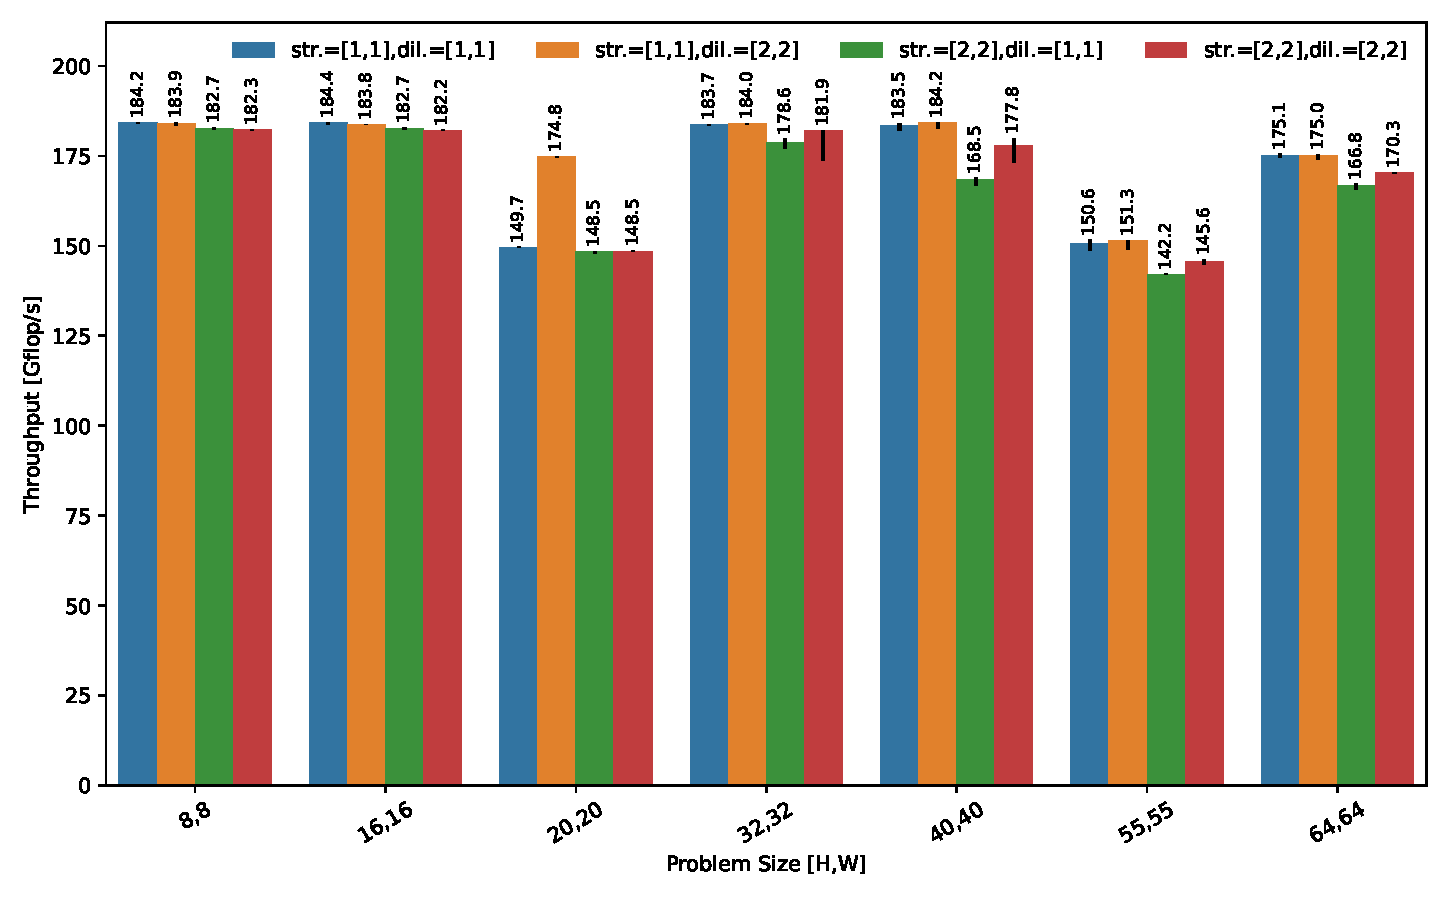
\includegraphics[width=0.98\textwidth]{plots/conv/conv_2d.pdf}
\endminipage
\caption{\label{fig:conv-2d} L1-resident $2$-D convolution for different strides, dilations, and problem sizes ($(N,C,F,K_h,K_w)$ fixed to $(1,32,64,3,3)$). 
Theoretical peak is $192 \mathrm{GFLOP}/s$, fine tuning of performance is left for future work.}
\end{figure}

Since this is a heavily compute-bound kernel with multiple parameters, we only focus on the performance of the vectorized kernel for small sizes resident in L1.
Thanks to our modular and composable approach, larger sizes can be built from smaller sizes, following previously discussed padding, packing and peeling strategies (see Section~\ref{subsec:padding-values-and-packing}).
In particular, the compiler implements a single $1$-D vectorization strategy that exhibits enough arithmetic intensity and is reused in the $2$-D case.
To achieve this, the $2$-D strategy simply tiles the $H$ and $K_h$ dimensions by $1$ then folds and canonicalizes it further.
The $2$-D case reduces to the $1$-D case where high-intensity vectorization patterns apply.

\subsection{Depthwise Convolution}

Depthwise convolution is a compute-efficient twist on convolution mainly oriented at mobile inference.
$1$-D and $2$-D depthwise convolution in \lstinline|NHWC| format are expressed as:
\begin{equation*}
\begin{array}{llll}
O[n,w,c] &=& I[n,w\times S_w+k_w\times D_w,c]\cdot K[k_w,c] & (1-D) \\
O[n,h,w,c] &=& I[n,h\times S_h+k_h\times D_h,w\times S_w+k_w\times D_w,c]\cdot K[k_h,k_w,c] & (2-D)
\end{array}
\end{equation*}
where the strides ($S_h$ and $S_w$) and the dilations ($D_h$ and $D_w$) control the input image access pattern. 
Compared to classical convolutions, the volume of the computation kernel is reduced by $1$ dimension (typically a $16\times$ to $512\times$ reduction in both compute and data volume).
The computation is also altered to only reduce across the window dimension(s) (and not along the channel dimension).
The depthwise convolution kernel has a low arithmetic intensity ($\frac{K_w}{\mathrm{sizeof}(\mathrm{element\_type})}$ $\mathrm{FLOP}/s$ per byte in the $1$-D case and $\frac{K_h.K_w}{\mathrm{sizeof}(\mathrm{element\_type})}$ $\mathrm{FLOP}/s$ per byte in the $2$-D case).
As a result, depthwise convolution is memory bandwidth-bound on modern server processors.

Since the kernel is memory-bound, it is important to measure the volume of data properly.
In the following experiments, we evaluate the total data volume as follows ($K_h$ and $H$ are $1$ in the $1$-D case):
\begin{equation*}
\begin{array}{lll}
\mathrm{Total}_{\mathrm{size}} &=& \mathrm{Out}_{\mathrm{size}} + \mathrm{Ker}_{\mathrm{size}} + \frac{\mathrm{In}_{\mathrm{size}}}{\Pi_i \gcd(\mathrm{stride}_i, \mathrm{dilation}_i)} \\
           &=& N\cdot C\cdot 
                \left(H\cdot W + \frac{H_{\mathrm{in}} \cdot W_{\mathrm{in}}}{\Pi_i \gcd(\mathrm{stride}_i, \mathrm{dilation}_i)}\right) + K_h\cdot K_w\cdot C 
\end{array}
\end{equation*}
The conservative reasoning follows:
\begin{enumerate}
    \item Every element of the convolution kernel is read.
    \item Every element of the output is written but is not considered read; the data is simply overwritten.
    \item Only a subset of the input is read, depending on the values of the stride and dilations quantities. This is captured by a scaling \emph{adjustment} factor.
\end{enumerate}
The scaling adjustment factor is obtained by the intersection of the stride lattice and the dilation lattice, within the limits of the input boundary.
The gcd is a good approximation when the size of the kernel is greater than the stride.
This guarantees we only compute the input points that participate in the derivation of at least $1$ output element.
This is a conservative measure: any element that is unused but falls in a common cache line with a used element is not counted; still the data will be moved by the hardware.

Figures~\ref{fig:depthwise-conv-1d} and~\ref{fig:depthwise-conv-2d} show the memory bandwidth for the $1$-D and $2$-D depthwise convolution.
All problem sizes not shown in the plot are constant ($(N,C,K_w)=(1,32,3)$ for the $1$-D case and $(N,C,K_h,K_w)=(1,32,3,3)$ for the $2$-D case).
In the $1$-D case, we measure $45-75\%$ L1 bandwidth for the smaller problem sizes compared to \emph{Copy2D}.
As size increases, we see performance close to the L2 and L3 bandwidth of \emph{Copy2D}, which signals strong data reuse.
For the $2$-D case, we limit the exploration to sizes related to MobileNet layers with batch size $1$. 
We again see performance within $10-20\%$ of the peak L3 bandwidth for comparable sizes, suggesting good data reuse.

\begin{figure}[h!tb]
\centering
\minipage[t]{\textwidth}
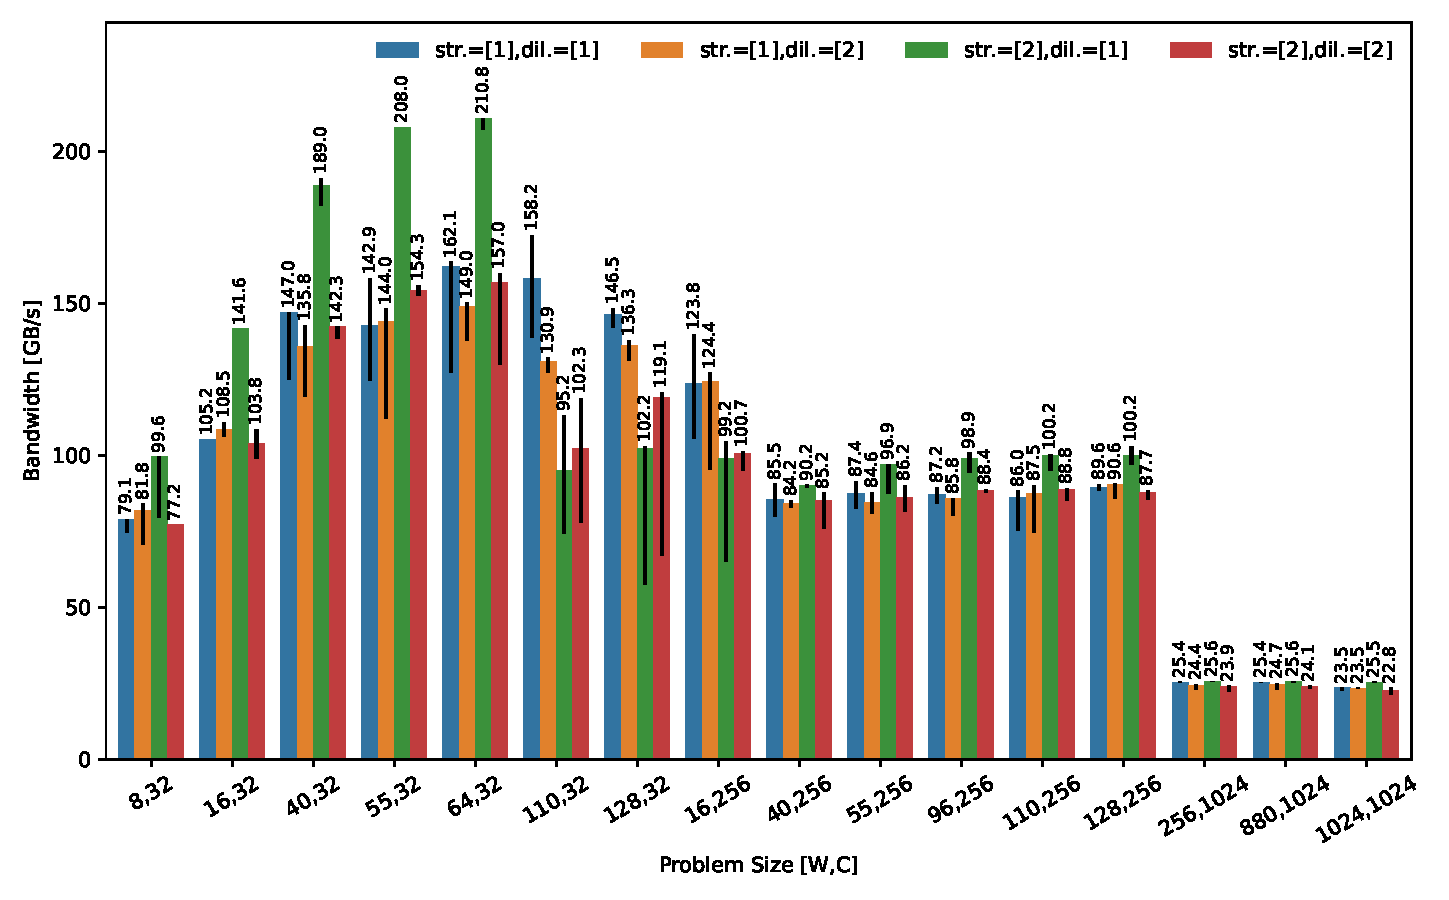
\includegraphics[width=0.98\textwidth]{plots/depthwise_conv/depthwise_conv_1d.pdf}
\endminipage
\caption{\label{fig:depthwise-conv-1d}1-D depthwise convolution for different strides, dilations, and problem sizes. Measured copy peak $289 \mathrm{GB}/s$ (L1), $89.3 \mathrm{GB}/s$ (L2), $25.7 \mathrm{GB}/s$ (L3 @40\%).}
\end{figure}

\begin{figure}[h!tb]
\centering
\minipage[t]{\textwidth}
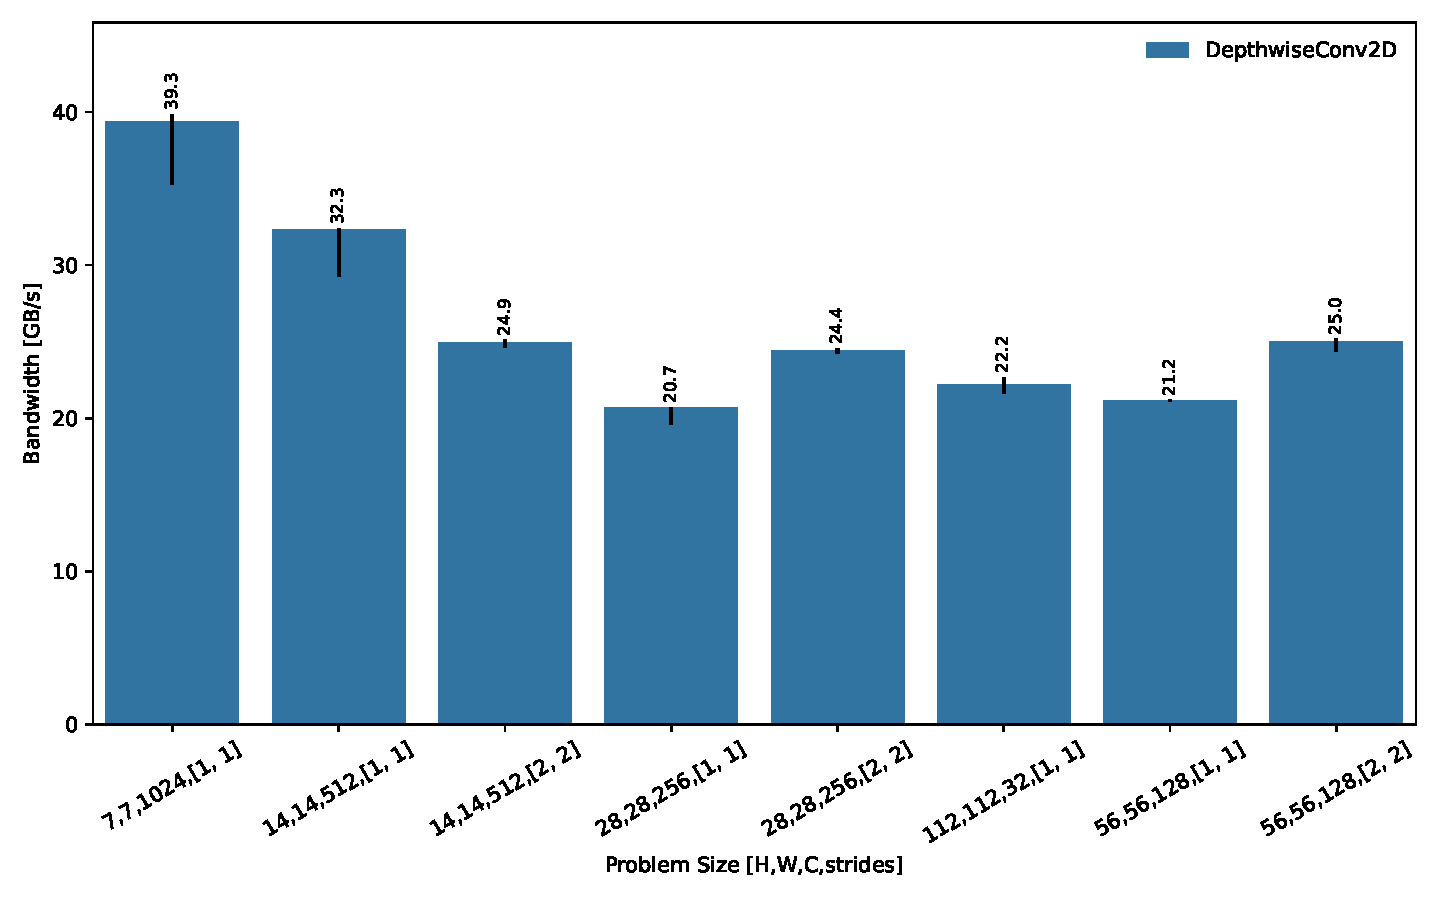
\includegraphics[width=0.98\textwidth]{plots/depthwise_conv/depthwise_conv_2d.pdf}
\endminipage
\caption{\label{fig:depthwise-conv-2d}2-D depthwise convolution for different strides, dilations, and problem sizes. Measured copy peak $54.8 \mathrm{GB}/s$ (L2 @90\%), $25.7 \mathrm{GB}/s$ (L3 @40\%). The \lstinline|7x7x1024| problem takes \lstinline|16x16x1024xf32=1.05M| (input and output tensors). This slightly exceeds L2. Other sizes are deep in L3 territory and require parallelism to increase bandwidth (outside the scope of this paper).}
\end{figure}

Lastly, note that our approach scales easily to other kernel sizes, strides and dilations than the traditional $1$ or $2$ values that are 
often the only supported by library implementations (and often not in all combinations).

\subsection{A Brief Evaluation of Sparse Code Generation}

We end this experimental evaluation with an example of sparse tensor code generation. As stated earlier, the \lstinline{sparse_tensor} dialect introduces the concept of sparse compilation into MLIR. The dialect makes sparse tensor types first class citizens by bridging high-level operations on these sparse tensors types with lower-level operations on the actual sparse storage schemes. To this end, the sparse tensor dialect introduces a tensor encoding attribute that allows specifying the formats of the Tensor Algebra Compiler (TACO)~\cite{kjolstad2017taco}. 

Figure~\ref{fig:sparse_layouts} illustrates how to use the the well-known Doubly Compressed Sparse Column (DCSC) storage format for sparse matrices in a matrix multiplication. A sparse tensor is specified by simply placing the encoding attribute inside the tensor type. This way of defining sparse tensor formats is quite powerful. 
For a single $d$-dimensional tensor, the dimension level formats and ordering alone give rise to $2^d \cdot d!$ different formats. 
This allows annotating a sparse kernel in a such a way that eventually results in the generation of effective sparse code. Even the output tensor could be made sparse to save memory when storing the result.

A set of \lstinline{sparse_tensor} dialect rewrite rules take care of lowering the kernel to sparse storage schemes and imperative constructs that only store and iterate over the nonzero elements to perform the matrix multiplication. Such an approach to automatic sparse code generation was first proposed in~\cite{bik96,biktms} in the context of sparse linear algebra, and later generalized to sparse tensor algebra in~\cite{kjolstad2017taco}. Even though the details of these rewrite rules are outside the scope of this paper, they follow a similar high-level modular and composable philosophy as discussed in Section~\ref{sec:transformations}, with variations in the transformations due to the use of sparse index sets and slightly more complicated bufferization due to the compound nature of sparse storage schemes. The rewrite rules similarly interoperate with \lstinline|linalg|, \lstinline|tensor|, \lstinline|memref|, \lstinline|scf|, and \lstinline|vector| abstractions, thereby progressive lowering a sparsity agnostic definition of a kernel into a form that fully exploits the sparsity of tensors as well as all performance features of the target architecture.

Consider, for example, a matrix times vector computation \texttt{x = Ab} for a general sparse matrix \texttt{A} (Figure~\ref{fig:sparse_lowering}). When \texttt{A} is in Compressed Sparse Row (CSR) format, nested \lstinline|scf| loops are used to iterate over the outer dense dimension, and, by means of an indirection, just the nonzero elements of the compressed inner dimension. 

\begin{table}[h!tb]
  \small
  \centering
  \begin{tabularx}{\textwidth}{X|rr|rr}
    \toprule
    \textbf{Size} & TACO random    & MLIR random   & TACO column        & MLIR column \\
    \midrule
    \lstinline|16,384 x 16,384| &  3.32 &  2.93 &  1.96 &  1.58 \\
    \lstinline|32,768 x 32,768| & 12.71 & 12.59 &  8.12 &  6.90 \\
    \lstinline|65,536 x 65,536| & 51.49 & 50.48 & 32.21 & 30.48 \\
    \bottomrule
  \end{tabularx}
  \smallskip
  \caption{Sparse kernel runtimes (in ms) on an Intel Xeon W2135 $3.7\mathrm{GHz}$.}
  \label{tbl:sparse-matvec}
\end{table}

\begin{figure}[h!tb]
    \centering
    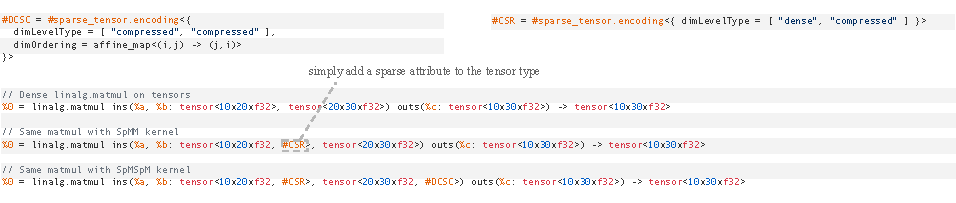
\includegraphics[width=\textwidth]{figures/sparse_layouts}
    \caption{Definition of sparse tensor layouts and their usage in a matrix multiplication.}
    \label{fig:sparse_layouts}

    \medskip
    \centering
    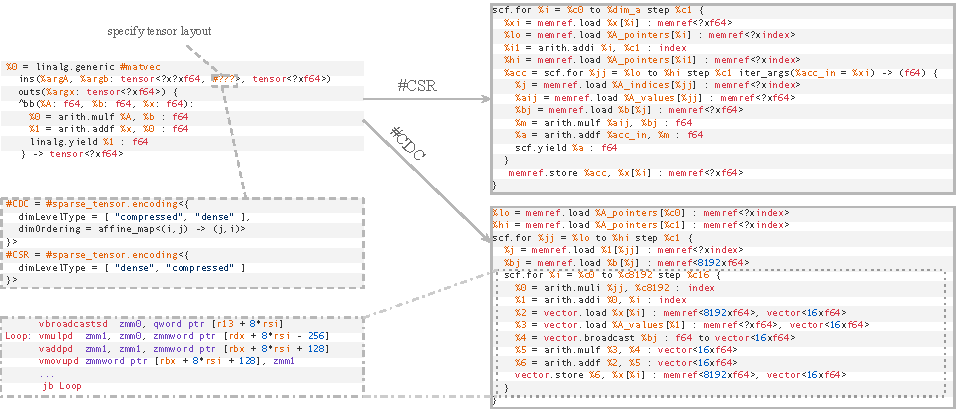
\includegraphics[width=\textwidth]{figures/sparse_lowering.pdf}
    \caption{Example: lowering of matrix-vector multiplication with sparse input matrix.}
    \label{fig:sparse_lowering}
\end{figure}

Now suppose that the sparse matrix \texttt{A} is actually a structured sparse matrix, where most columns are empty, but when nonzero, the columns are dense, i.e.\ mostly filled. In that case, \texttt{CDC} makes more sense, favoring column-wise access over the default row-wise storage, and using compression for the outermost dimension (now columns) only. Specializing for this format for a sparse $8192 \times 8192$ matrix and a vector length of 16, the sparse rewriting rules compose well with vectorization to eventually yield sparse vector code that skips over empty columns, but performs the innermost dense update using vectors. After more progressive lowering within MLIR, eventually an LLVM IR representation is handed off to the backend compiler which, when targeting AVX512, generates an innermost loop that performs the vector updates in full SIMD.

Table~\ref{tbl:sparse-matvec} shows the runtime (in ms) on an Intel Xeon W2135 $3.7\mathrm{GHz}$, comparing sparse computations generated by both TACO and MLIR, evaluated on sparse matrices with a random uniform density of about 1\% (random) and matrices with 1\% of the columns filled (column). For TACO, we used the default settings of the built-in benchmark, but excluded compilation time for a fair comparison. The table clearly shows that the sparse compiler component of MLIR is on-par with a state-of-art compiler like TACO, with additional benefits when the transformation of MLIR's sparse compiler are composed with other optimizations, such as vectorization.

\subsection{Preliminary Autotuning Results}
\label{subsec:prelim-tuning-results}

Our collaborators at Nod.AI have been using our modular and composable codegen strategy and tuning it for specific use cases. 
They have built an autotuner using CompilerGym~\cite{CompilerGym}, a compiler tuning environment based on the OpenAI Gym~\cite{OpenAIGym}.
They report fully-automatic preliminary results on recent Alder Lake CPUs~\cite{NodeAi-tuner} on which they outperform both Intel's MKL library and the TVM autotuner on a variety of matrix multiplication sizes relevant to the machine learning community.
When integrated within the IREE~\cite{iree} compiler-based runtime system, and further tuned for a BERT~\cite{Bert} model on NVIDIA A100 GPUs, they report the fastest end-to-end PyTorch-based~\cite{PyTorch} inference numbers~\cite{NodeAi-runtime}.
